\documentclass[standalone, version=2.0]{huangfusl-template}
\begin{document}
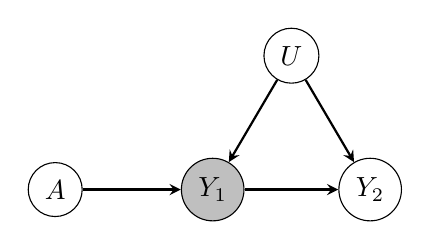
\begin{tikzpicture}
    \node[circle, draw, fill=gray!50!white] (Y1) at (2, 0) {$Y_1$};
    \node[circle, draw] (A) at (0, 0) {$A$};
    \node[circle, draw] (Y2) at (4, 0) {$Y_2$};
    \node[circle, draw] (U) at (3, 1.7) {$U$};

    \draw[-stealth, thick] (A) -- (Y1);
    \draw[-stealth, thick] (Y1) -- (Y2);
    \draw[-stealth, thick] (U) -- (Y1);
    \draw[-stealth, thick] (U) -- (Y2);
\end{tikzpicture}
\end{document}